\documentclass[titlepage=firstiscover, bibliography=totoc, captions=tableheading, parskip=half]{scrbook}
\titlehead{
  \centering
  
\includegraphics[scale=2.3]{pics/logo.png}
}
\author{Felix Geyer \\
  \texorpdfstring{\href{mailto:felix.geyer@tu-dortmund.de}{felix.geyer@tu-dortmund.de}}{}
  }
\title{Projektbericht zum Seminar: Maschinelles Lernen}
\publishers{TU Dortmund - Fakultät Physik}
\date{Abgabe: 15. Februar 2019}
\usepackage[aux]{rerunfilecheck}
\usepackage{polyglossia}
\setmainlanguage{german}
\usepackage{amsmath}
\usepackage{amssymb}
\usepackage{mathtools}
\usepackage{fontspec}
\usepackage[version=4]{mhchem}
\usepackage{scrhack}
\usepackage{float}
\floatplacement{table}{htbp}
\floatplacement{figure}{htbp}

\usepackage[locale=DE, separate-uncertainty=true, per-mode=reciprocal, decimalsymbol=comma]{siunitx}
%\usepackage{siunitx}
\DeclareSIUnit\px{px}

\usepackage[sorting=none]{biblatex}
\addbibresource{content/lit.bib}

\usepackage[section, below]{placeins}
\usepackage[labelfont=bf,
font=small,
width=0.9\textwidth,
format=plain,
indention=1em]{caption}
\usepackage{graphicx}
\usepackage{grffile}
\usepackage{subcaption}

\usepackage[math-style=ISO, bold-style=ISO, sans-style=italic, nabla=upright, partial=upright]{unicode-math}
\setmathfont{Latin Modern Math}

\usepackage[autostyle]{csquotes}

\usepackage[unicode]{hyperref}

\usepackage{mathtools}
\DeclarePairedDelimiter\abs{\lvert}{\rvert}

\usepackage{bookmark}

\usepackage{booktabs}

\usepackage{rotating}

\usepackage{tikz}
\usetikzlibrary{positioning}

\newcommand\JPsi{$J/\Psi$}
\newcommand\zerfall{$\beta$-Zerfall }
\newcommand\zerfalls{$\beta$-Zerfalls}
\newcommand\SppS{$\symup{Sp\bar{p}S}$}
\newcommand\barparen[1]{\overset{(-)}{#1}}

\begin{document}

\maketitle
  \section{Definition und Motivation}
  \begin{frame}{Definition und Motivation}
    Fragestellung:
    \begin{center}
      \textbf{Wie schnell und präzise kann eine Hunderassen-Klassifizierung mit 120 Klassen
      durchgeführt werden?}
    \end{center}
    Motivation:
    \begin{itemize}\setlength\itemsep{1em}
      \item Klassifizierung ohne Vorwissen möglich
      \item Persönliche Defizite ausgleichen
      \item Hunde sind cooler als Katzen
    \end{itemize}
  \end{frame}
  \section{Datensatz}
  \begin{frame}{Datensatz}
    \begin{itemize}\setlength\itemsep{1em}
      \item \href{https://www.kaggle.com/jessicali9530/stanford-dogs-dataset}{Stanford Dogs Dataset}
      \item Lizenz: ???
      \item Informationen: Klassifikationen und Bounding Boxes
      \item Anzahl Einträge: 20.580 auf 120 Klassen verteilt
      \item Input-Features: Bilder
      \item Target-Variablen: Klassen und Bounding Boxes
      \item Bisherige Arbeiten: Kernels bei Kaggle
    \end{itemize}
  \end{frame}

  \section{Alternativ-Methode}
  \begin{frame}{Alternativ-Methode}
    \begin{columns}[c]
      \column{0.6\textwidth}
      \begin{itemize}\setlength\itemsep{2em}
        \item \textbf{Ziel:} Vergleich zweier Architekturen \\
        \rightarrow \ CNN ohne Bounding Boxes und ein vorgeschaltetes CNN, welches
        die Bounding Boxes predicted
        \item \textbf{Motivation:}
        \begin{itemize}\setlength\itemsep{1em}
          \item Ohne Bounding Boxes: besser für allgemeine und schnelle
          Verwendbarkeit
          \item Allerdings: Klassifizierung mit Bounding Boxes sollte besser funktionieren,
          da weniger störanfällig
        \end{itemize}
      \end{itemize}
      % Wir wollen zwei Architekturen vergleichen, ein CNN ohne Bounding Boxes und zwei
      % CNN, bei welchen das erste die Bounding Boxes predicted und damit dann das zweite
      % CNN ausführt, welches die Klassifizierung vornimmt. Motivation: Es wäre besser
      % für die allgemeine und schnelle Verwendbarkeit, allerdings sollte die Klassifizierung
      % mit Bounding Boxes besser funktionieren, da sie weniger störanfällig ist.
      \column{0.4\textwidth}
      \begin{figure}
        \centering
        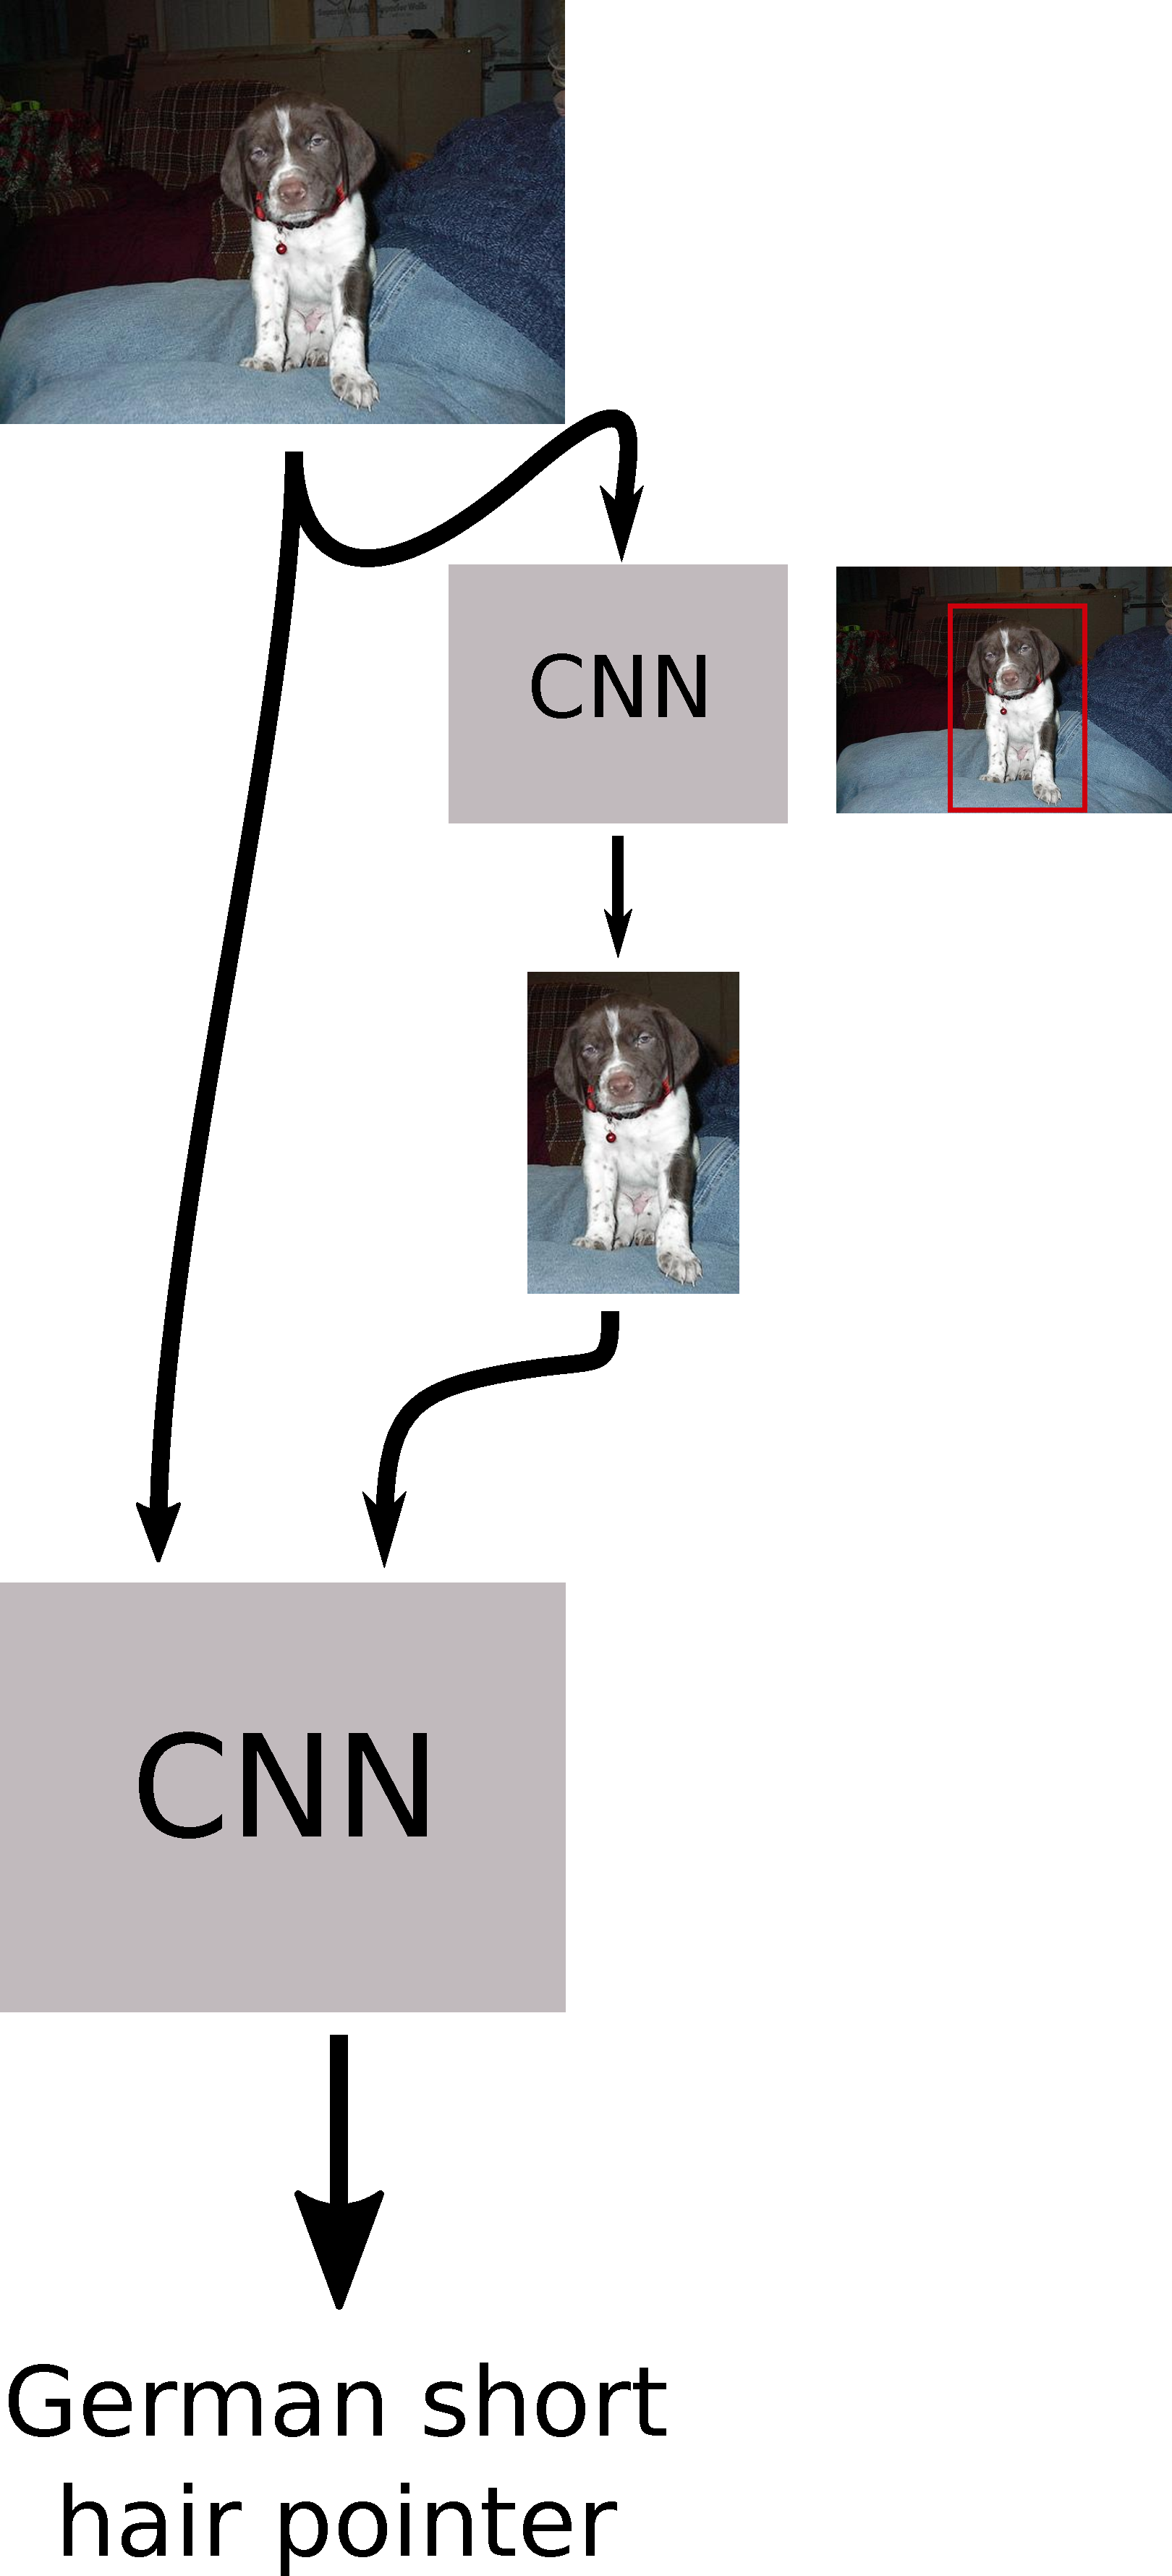
\includegraphics[width=0.6\textwidth]{logos/alternative_method.pdf}
        \caption{Blau: Ohne Verwendung von Bboxes. \quad Orangefarbend: Verwendung von BBoxes}
        %\label{}
      \end{figure}
    \end{columns}
  \end{frame}
\end{document}
